\begin{figure*}[t!]

\centering
\begin{minipage}{.5\textwidth}
  \centering
  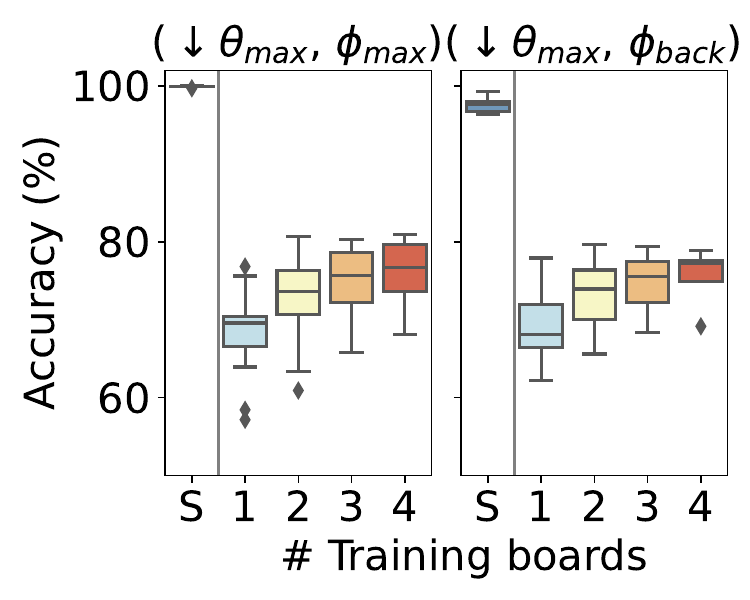
\includegraphics[width=0.90\linewidth]{fig/combo-nobacksub-and-backsub-acc-big.png}
  {\label{fig:multi-board-acc}}
\end{minipage}%
\begin{minipage}{.5\textwidth}
  \centering
  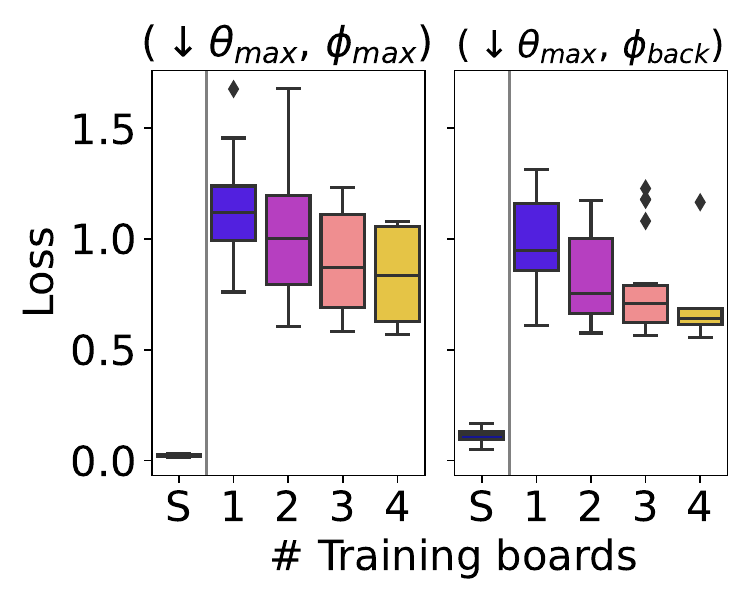
\includegraphics[width=0.90\linewidth]{fig/combo-nobacksub-and-backsub-loss-big.png}
  {\label{fig:multi-board-loss}}
\end{minipage}
\vspace{-10pt}
% \subfigure%[\hspace{15pt}Accuracy Boxplot]
% {\label{fig:multi-board-acc}
% \vspace{-50pt}
% 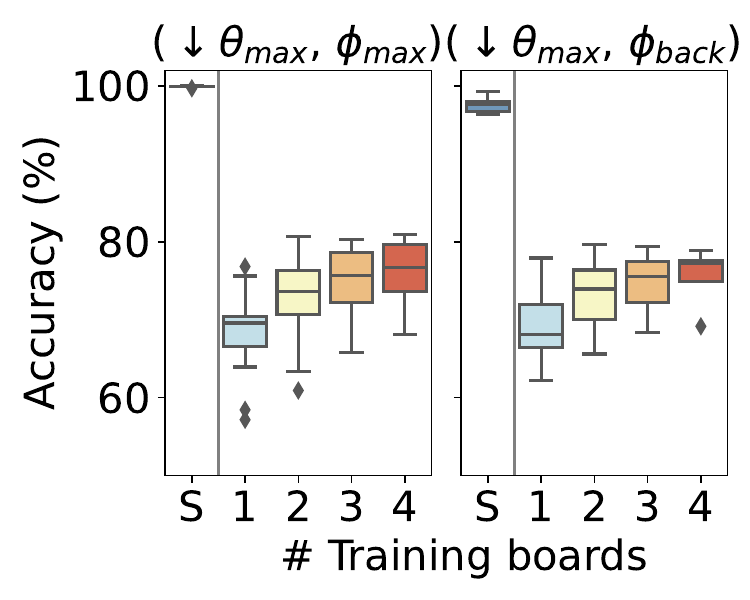
\includegraphics[width=0.55\columnwidth]{fig/combo-nobacksub-and-backsub-acc-big.png}
% }\\
% \vspace{-15pt}
% \subfigure%[\hspace{12pt}Loss Boxplot]
% {\label{fig:multi-board-loss}
% 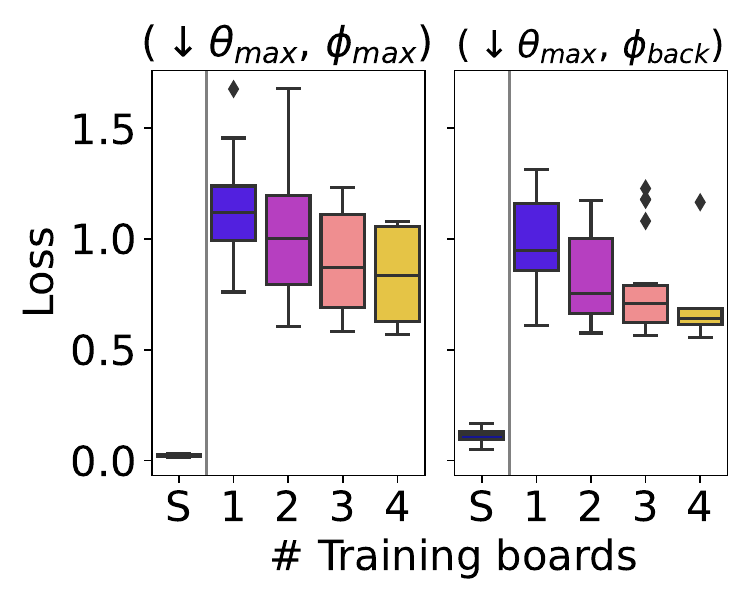
\includegraphics[width=0.55\columnwidth]{fig/combo-nobacksub-and-backsub-loss-big.png}}
% \vspace{-20pt}
\caption{Multi-board Training and Inference Results. Plots show Accuracy and Loss when training on 1-4 boards with background subtraction ($\downarrow\theta_{max}$, $\phi_{back}$) and without ($\downarrow\theta_{max}$, $\phi_{max}$). 
Testing always occurs on data from a separate board, except for when data from the same board is used (denoted ``S''). Background subtraction decreases the cross-board accuracy's interquartile range (IQR) by 2.3$\times$ and the loss's IQR by 5.8$\times$. 
Multi-board training and background subtraction greatly improve cross-board generalization.} 
\label{fig:multi-board}
\vspace{-10px}
\end{figure*}
